\begin{problem}
Find an example of a finitely generated ring extension $R\subset
S$ where $S$ is a Noetherian ring, but $R$ is not.
\end{problem}
\begin{proof}

\end{proof}
\newpage
\begin{problem}
Consider the homomorphism of rings
\begin{center}
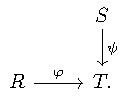
\includegraphics{figures/hw-4-ring-maps}
\end{center}
The \emph{fiber product} of $R$ and $S$ over $T$ is the subring
$R\times_T S=\left\{\,(r,s)\;\middle|\;\phi(t)=\psi(s)\,\right\}$
of $R\times S$. Assume $\phi$ and $\psi$ are surjective. Show
that if $R$ and $S$ are Noetherian rings then so is $R\times_T
S$.
\end{problem}
\begin{proof}
\end{proof}
\newpage
\begin{problem}
Let $M$ be an $R$-module. Show that $M$ is a flat $R$-module if
and only if $M_{\mathfrak{m}}$ is a flat
$R_{\mathfrak{m}}$-module for every maximal ideal $\mathfrak{m}$
of $R$.
\end{problem}
\begin{proof}
\end{proof}
\newpage
\begin{problem}
Let $M$ be an $R$-module and $\mathfrak{a}$ an $R$-ideal.
\begin{enumerate}[noitemsep,label=(\alph*)]
\item Show that if $M_{\mathfrak{m}}=0$ for every maximal ideal
  $\mathfrak{m}$ containing $\mathfrak{a}$, then $M=IM$.
\item Show that the converse holds in case $M$ is finite.
\end{enumerate}
\end{problem}
\begin{proof}
\end{proof}
\newpage
\begin{problem}
Prove that every power of a maximal ideal is primary.
\end{problem}
\begin{proof}
\end{proof}
\newpage
\begin{problem}
\begin{enumerate}[noitemsep,label=(\alph*)]
\item Show that the radical of a primary ideal is prime.
\item Find an example of a power of a prime ideal that is not
  primary.
\item Let $\mathfrak{p}$ be a prime ideal of a ring $R$ and
  $n\in\NN$. The $R$-ideal
  $\mathfrak{p}^{(n)}=R\cap\mathfrak{p}^nR_{\mathfrak{p}}$ s
  called the \emph{$n$th symbolic power of $\mathfrak{p}$}. Show
  that $\mathfrak{p}^{(n)}$ is primary.
\end{enumerate}
\end{problem}
\begin{proof}
\end{proof}

%%% Local Variables:
%%% mode: latex
%%% TeX-master: "../MA557-HW-Current"
%%% End:
